\documentclass[../rapport.tex]{subfiles}
\graphicspath{{\subfix{ressources/photos_diagrammes/extensionThomas/}}}

\begin{document}
		\subsubsection{Vue d'ensemble}
		Le but de cette extension est de rajouter la gestion de contrats d'assurances divers
		à la fois pour les client smais égalemet pour les insitutions. L'extension se base tout
		de même sur la structure de l'application 1 car c'est dans celle-ci qu'elle la plus 
		utilisée. En effet, dans l'appliction 2 elle est gére comme les autres produits 
		financiers. Il n'y a réellement que la réponse à une demande de devis qui diffère.
		Afin de rendre les diagrammes plus visibles j'ai changé les couleurs des éléments rajoutés. 
		Rose pour le diagramme d'entité relation et jaune pour les autres diagrammes.

		\subsubsection{Application 1}

		\subsubsection{Diagramme des cas d'utilisation}
				\begin{figure}[h]
						\centering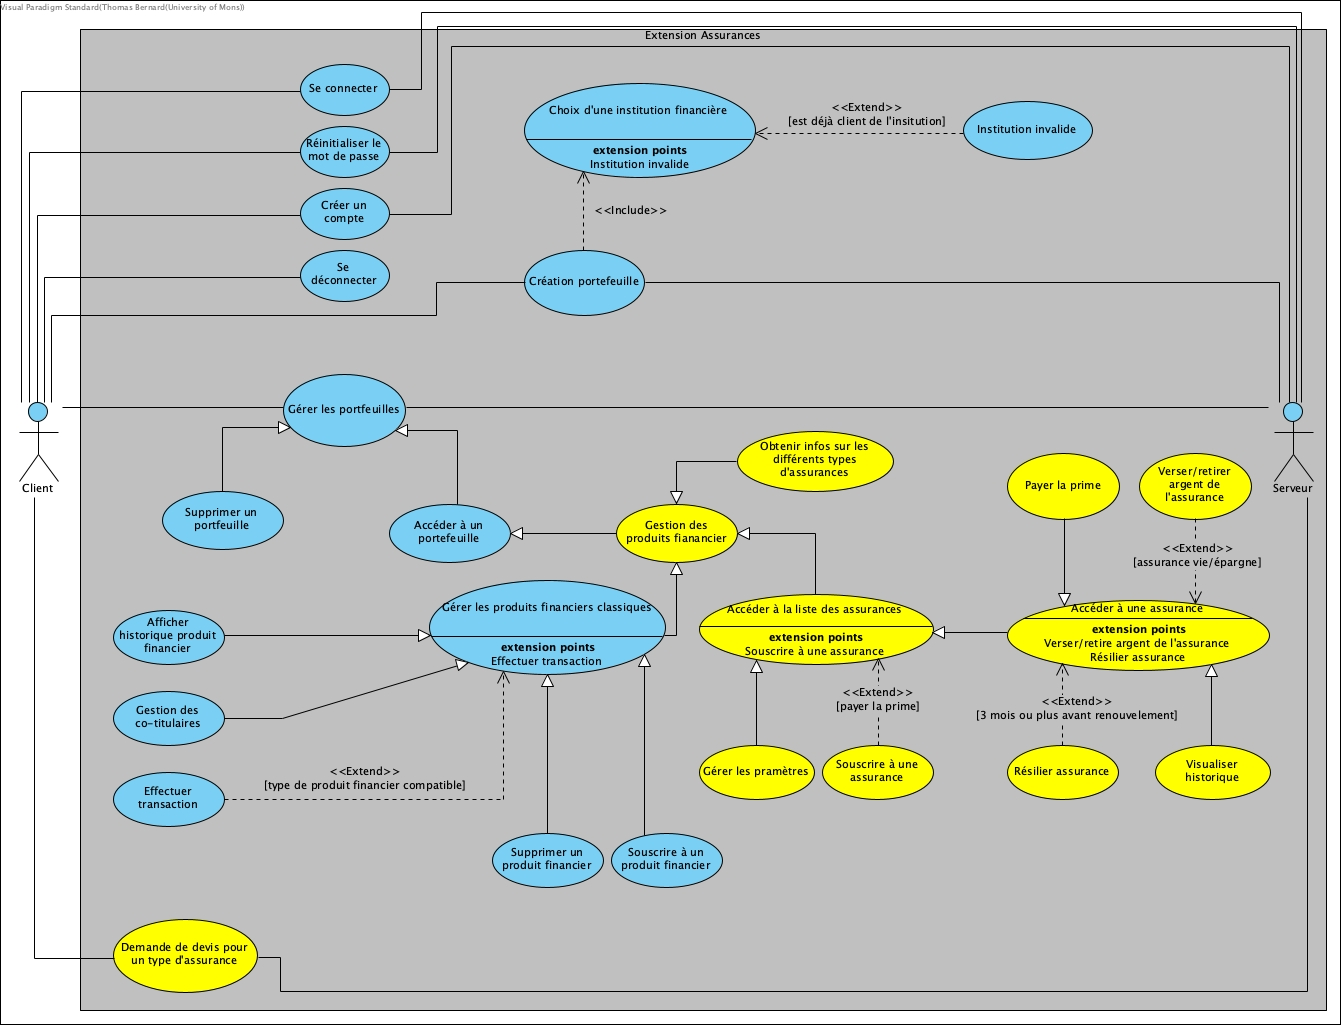
\includegraphics[scale=0.27]{ressources/photos_diagrammes/extensionThomas/useCase1Thomas.jpg}
						\caption{Diagramme des cas d'utilisation de l'app 1 avec extension}
				\end{figure}
		J'ai rajouté un ensemble de divers cas d'utilisations qui sont propres aux assurances
		mais toutefois semblables aux cas d'utilisation relatifs aux produits financiers
		classiques. Il n'y a aucune remarque particulière à faire concernant les cas
		d'utilisation car le modèle est calqué sur le diagramme de base.
\newpage
		\subsubsection{Interaction Overview Diagram}
				\begin{figure}[h]
						\centering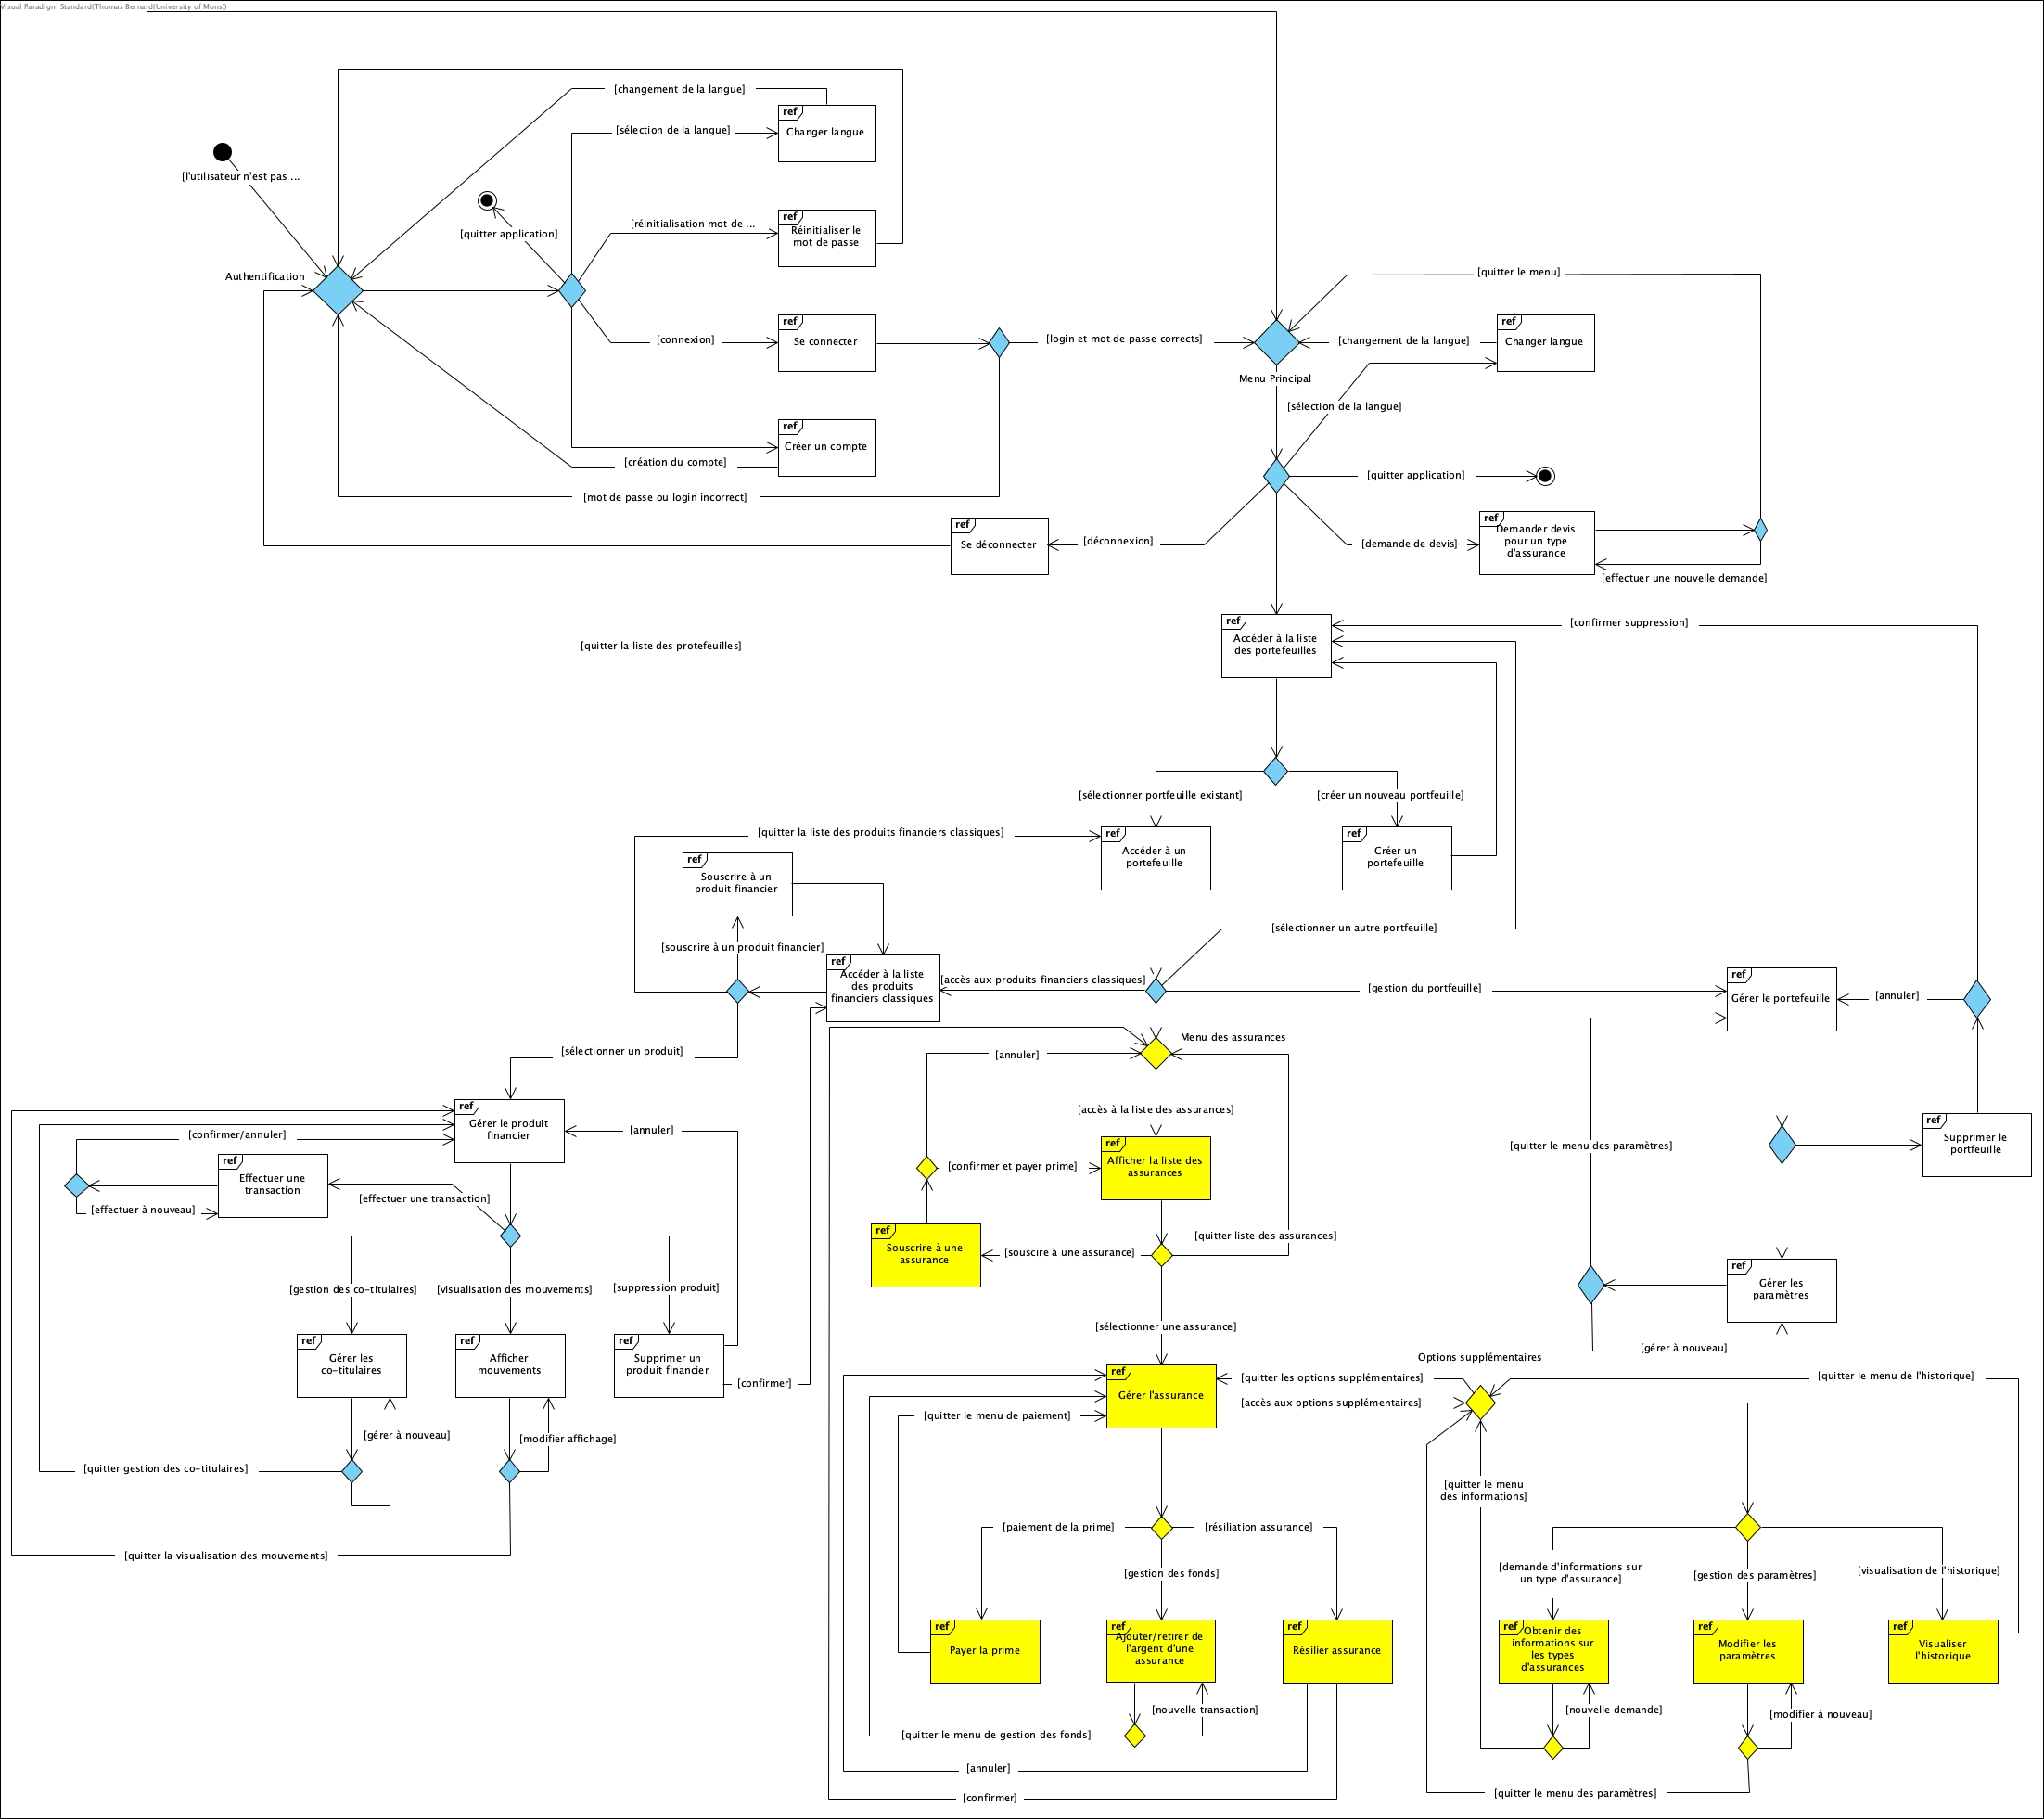
\includegraphics[scale=0.15]{ressources/photos_diagrammes/extensionThomas/intOver1Thomas.jpg}
						\caption{Interaction Overview Diagram de l'app 1 avec extension}
				\end{figure}
		Encore une fois ce diagramme se base sur celui de l'application 1. Notons qu'il est
		maintenant possible de demander un devis depuis le menu principal. Il y a également une 
		différenciation entre les produits financiers classiques et les assurances afin de les 
		séparer en deux scènes différentes plus tard dans la GUI.

\newpage
		\subsubsection{Diagrammes de classe}
				\begin{figure}[h]
						\centering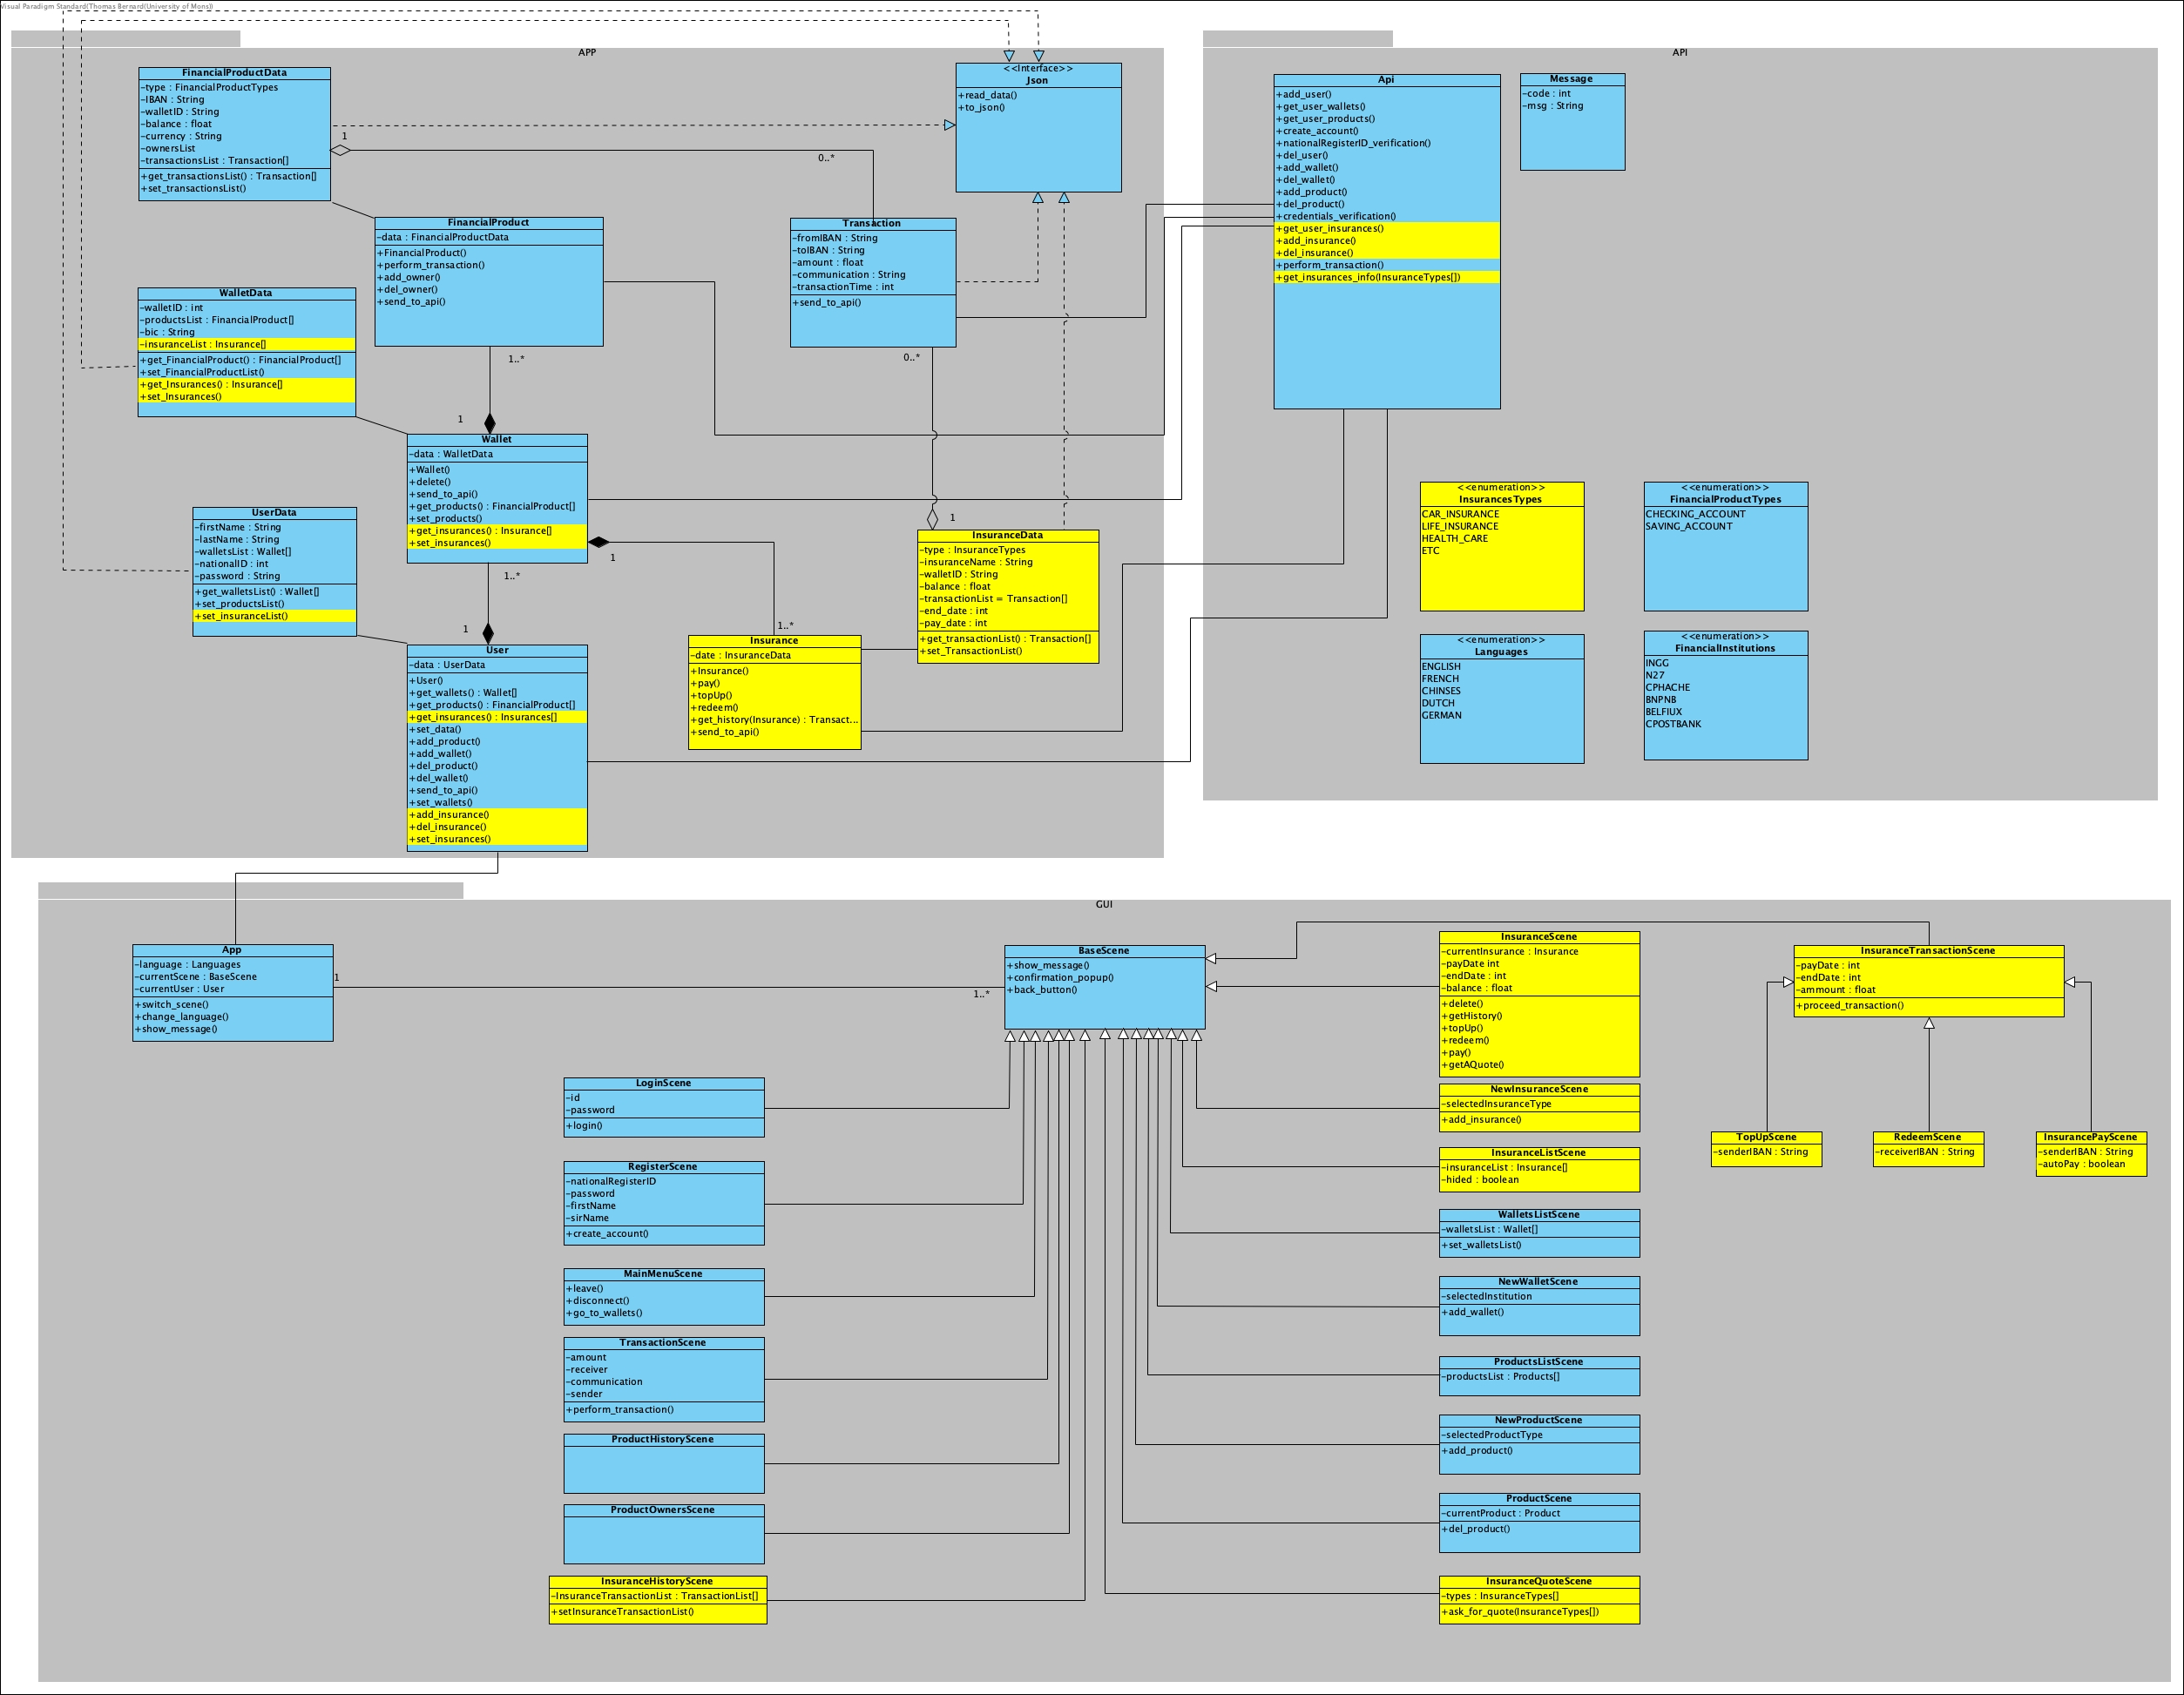
\includegraphics[scale=0.15]{ressources/photos_diagrammes/extensionThomas/class1ExtensionThomas.jpg}
						\caption{Diagramme de classes de l'app 1 avec extension}
				\end{figure}
		Dans la partie logique de l'application (package APP) deux classes ont été rajoutées :
		\textbf{Insurance} et \textbf{InsuranceData}. La première contioent le constructeur et 
		un attribut \textit{data} qui est une objet de type \textit{InsuranceData}. La classe 
		contient également les méthodes liées aux assurances. La classe \textbf{Insurance} est
		liée à la classe wallet de même manière que la classe \textbf{FinancialProduct}. 
		La classe \textbf{Insurance} possède une méthode \textit{send\_to\_api()} et est connectée 
		au package API. La classe \textbf{InsuranceData} implémente l'interface \textbf{Json} qui
		permet d'écrire et le dire des fichiers json de données et d'ainsir mettre ses données à
		jour.

		\medskip

		Les classes de bases dans lesquelles se trouvaient des listes de produits, des setter et 
		des getter se sont vues ajouter des setter, des getter et des listes mais cette fois-ci
		pour les assurances. 

		\bigskip

		Dans la partie serveur du diagramme de classe (package API) j'ai rajouté une enumération
		\textbf{InsurancesTypes} qui contient les différents types d'assurances afin de pouvoir
		interpréter correctment les données envoyées à la classe \textbf{Api}. Dans la classe
		\textbf{Api} des méthodes ont été rajoutées afin de pouvoir ajouter, supprimer et obtenir
		les assurances d'un client. Il y a également une méthode permettant d'obtenir des 
		informations sur un ou plusieurs types d'assurances dans le cadre de devis.

		\bigskip

		Dans la partie interface graphique (package GUI) il s'agit principalement de nouvelles 
		scènes rajoutées à la manière des scènes de l'application de base. Il n'y a pas de 
		point particulier à expliquer ici.
\newpage
\end{document}
